\subsubsection{类的基本概念}

类是\textbf{面向对象}（OO，Object-Oriented）最基本的概念，也是C++区别于C语言的重要特征。
面向对象编程的基本思想是抽象出对象，将对象作为程序的基本单元，通过消息传递来进行通信和协作。
对象是类的实例，具有状态和行为：状态存储在对象的数据成员中，行为由对象的成员函数实现。
面向对象编程的优点是代码的可重用性、可扩展性和可维护性都得到了提高。

在C++中，类是一种抽象数据类型，它定义了对象的行为和状态，并提供了对这些数据的访问接口。
类可以包含数据成员、成员函数、构造函数、析构函数等，其中能从外部访问的成员构成了类的接口，私有成员则留给类自己管理。
类可以派生出新的类，从而实现代码的重用和扩展。

类的语法看起来零碎，我们先用小程序把成员声明、创建对象和调用连起来。项目放在 \path{examples/class-basics-demo}，文件组成如下。每个 cpp 都有自己的 main，分别编译；不要把它们拼成一个文件。
\begin{lstlisting}[language={}]
class-basics-demo/
  README.md
  class-template.cpp
  constant-template.cpp
  constructors.cpp
  designated.cpp
  function-template.cpp
  inheritance.cpp
  operators.cpp
  overload.cpp
  skeleton.cpp
  static-friend.cpp
\end{lstlisting}
编译命令里，-std 指定 C++ 标准，-Wall/-Wextra 打开常用警告，-pthread 配置线程编译与链接；-o 指定临时输出文件。先进入项目目录，后面的源码名按当前示例替换。

\Needspace{9\baselineskip}
\begin{example}
类的基本结构（先认识成员，再创建对象调用）：
\lstinputlisting[language=C++,numbers=left,numberstyle={\color{gray}\tiny}]{examples/class-basics-demo/skeleton.cpp}

从本卷目录进入 \path{examples/class-basics-demo}，保存的源码就是 \texttt{skeleton.cpp}。
\begin{tbash}
g++ -std=c++17 -Wall -Wextra -pthread skeleton.cpp -o /tmp/cpp-demo
/tmp/cpp-demo
\end{tbash}
这里输出 1，说明对象已经构造，公有成员函数可以使用私有数据。
\end{example}

\begin{enumerate}
    \item \textbf{构造函数和析构函数}：负责对象的初始化和释放，构造函数与类同名，析构函数在类名前加 \texttt{\textasciitilde}，两者都不写返回类型。
    \item \textbf{成员函数}：实现类的行为，它们实现了类的功能。
    \item \textbf{数据成员}：存储类的数据信息。
\end{enumerate}

\begin{center}
    \begin{tabular}{cc}
        \toprule[1.5pt]
        修饰限定符 & 作用 \\
        \midrule[1pt]
        private & 该类的成员和友元可以访问 \\
        public & 可以被类外的其他函数或派生类中函数调用 \\
        protected & 该类的成员、友元与派生类按规则访问 \\
        \bottomrule[1.5pt]
    \end{tabular}
\end{center}

顺带一提，C++是一门\textbf{多范式}语言：既可以像C语言那样面向过程（数据和函数分离，通过函数调用组织逻辑），
也可以面向对象，还可以用模板进行泛型编程。本章后面的小节会逐一见到它们。

\begin{note}
\texttt{struct} 和 \texttt{class} 在 C++ 中几乎完全等价，\textbf{唯一的区别是默认权限}：
\texttt{struct} 的成员默认 \texttt{public}、默认公有继承；\texttt{class} 的成员默认 \texttt{private}、默认私有继承。
除此之外，\texttt{struct} 一样可以有构造函数、成员函数、继承和多态。
习惯上 \texttt{struct} 用于纯数据打包（如坐标点），\texttt{class} 用于需要封装的对象。
\end{note}

\textbf{番外：指名初始化（Designated Initializers）。}
对于下面这种成员公开、没有用户声明构造函数的简单结构体（聚合类型，Aggregate Type），C++20 允许在初始化时指名道姓地给成员赋值。
不过成员名仍要按声明顺序写，不能因为写了名字就随意调换；这里先认识最简单的用法：

\Needspace{9\baselineskip}
\begin{example}
指名初始化：
\lstinputlisting[language=C++,numbers=left,numberstyle={\color{gray}\tiny}]{examples/class-basics-demo/designated.cpp}


从本卷目录进入 \path{examples/class-basics-demo}，保存的源码就是 \texttt{designated.cpp}。
\begin{tbash}
g++ -std=c++20 -Wall -Wextra -pthread designated.cpp -o /tmp/cpp-demo
/tmp/cpp-demo
\end{tbash}
这里输出 1 3。把 .a、.b 的顺序调换后，C++20 编译应失败，名字不能替代顺序规则。
\end{example}

\begin{exercise}\label{ex:v1-cpp-point}

定义一个 \texttt{Point} 类，包含私有数据成员 \texttt{x}、\texttt{y}（\texttt{double} 类型），
编写含参构造函数和打印坐标的成员函数，并在 \texttt{main} 中创建两个点验证。
\end{exercise}

\subsubsection{静态和友元}

\textbf{静态成员}（static member）属于整个类，而不是某个具体对象。
无论创建多少个对象，静态成员在内存中只有一份，被类的所有对象共享，因此可以实现一些全局变量的功能。
普通静态数据成员在类内用 \texttt{static} 关键字\textbf{声明}，用到时在类外提供一次\textbf{定义}。
从 C++17 起，也可以写成 \texttt{inline static int count = 0;}，直接在类内定义。静态成员函数没有 \texttt{this}，不能直接访问某个对象的非静态成员。
这里的静态数据成员具有静态存储期，不会随着某一个对象的析构一起消失。

\textbf{友元函数}（friend function）：有时我们希望某个函数可以访问类的私有成员，但又不希望它成为类的成员函数。
这时可以在类的声明中用 \texttt{friend} 关键字把它声明为友元函数。友元函数不是类的成员，实现时不加类的作用域，
但可以访问类的私有成员。

\Needspace{9\baselineskip}
\begin{example}
静态成员与友元函数的用法：
\lstinputlisting[language=C++,numbers=left,numberstyle={\color{gray}\tiny}]{examples/class-basics-demo/static-friend.cpp}


从本卷目录进入 \path{examples/class-basics-demo}，保存的源码就是 \texttt{static-friend.cpp}。
\begin{tbash}
g++ -std=c++17 -Wall -Wextra -pthread static-friend.cpp -o /tmp/cpp-demo
/tmp/cpp-demo
\end{tbash}
两行都是 10，最后友元读到 42；两个对象访问的是同一份静态数据。
\end{example}

\begin{note}
友元函数不属于类，但它是类主动授予的访问接口，流插入运算符就经常这样写。
这就像给需要帮忙的人配一把钥匙：有明确用途可以给，不要为了省事把所有函数都声明成友元。
\end{note}

\begin{exercise}\label{ex:v1-cpp-count}

为 \texttt{Point} 类添加一个静态数据成员 \texttt{count}，在构造函数中令其加一、析构函数中令其减一，
在 \texttt{main} 中分不同作用域创建若干对象，打印 \texttt{count} 观察对象数量的变化。再在 static-friend.cpp 中调用静态成员函数，说明它为什么没有 this；指出 FriendFunction 访问私有成员的授权来自哪里。
\end{exercise}

\subsubsection{函数重载}
\textbf{函数重载（overload）}是指在同一个作用域中，存在多个同名函数，但它们的参数个数或参数类型不同。
函数重载的作用是为了使程序更加灵活，提高代码的可读性和可维护性。

在C++中，函数重载的规则是：
\begin{enumerate}
    \item 函数名相同；
    \item 参数个数不同，或参数类型不同。
\end{enumerate}

\Needspace{9\baselineskip}
\begin{example}
同名不同参的 \texttt{CalSum}：
\lstinputlisting[language=C++,numbers=left,numberstyle={\color{gray}\tiny}]{examples/class-basics-demo/overload.cpp}


从本卷目录进入 \path{examples/class-basics-demo}，保存的源码就是 \texttt{overload.cpp}。
\begin{tbash}
g++ -std=c++17 -Wall -Wextra -pthread overload.cpp -o /tmp/cpp-demo
/tmp/cpp-demo
\end{tbash}
两行分别是 3 和 4，整数参数与小数参数选择了不同重载。
\end{example}

在上例中，CalSum函数的两个版本参数类型不同，编译器会根据调用时传入的实参，自动选择最匹配的函数版本。

\begin{note}
\textbf{仅返回值不同不能构成重载}。调用函数时编译器看不到你打算把结果赋给什么类型，
如果只靠返回值区分，这两个声明本身就会冲突，不能等调用时再靠接收结果的变量区分。
\end{note}

\begin{exercise}
\label{ex:v1-cpp-overload}
把 overload.cpp 的两个调用换成同类型的另一组参数，核验选择的版本；再在练习副本中只改变返回类型、保留相同参数列表，记录编译失败的原因。
\end{exercise}

\subsubsection{构造函数}

\textbf{构造函数的类型：}

\begin{enumerate}
    \item 默认构造：默认构造函数是指可以不提供实参就调用的构造函数（没有参数，或所有参数都有默认值），它会创建一个对象，并对其进行初始化。
    \item 含参构造：含参构造函数是指有参数的构造函数，可以根据参数的值对对象进行初始化。
    \item 拷贝构造：拷贝构造函数是指将一个对象拷贝到另一个对象时，会调用拷贝构造函数。
\end{enumerate}

\Needspace{9\baselineskip}
\begin{example}
三种构造函数的调用时机，注意每一次的输出：
\lstinputlisting[language=C++,numbers=left,numberstyle={\color{gray}\tiny}]{examples/class-basics-demo/constructors.cpp}


从本卷目录进入 \path{examples/class-basics-demo}，保存的源码就是 \texttt{constructors.cpp}。
\begin{tbash}
g++ -std=c++17 -Wall -Wextra -pthread constructors.cpp -o /tmp/cpp-demo
/tmp/cpp-demo
\end{tbash}
依次看到默认、含参、拷贝构造的提示；最后三个 member 分别为 10、2、10。
\end{example}

有一些tips可以快速设置构造函数：
\begin{tcode}
ClassName() = default;              //默认构造函数,使用默认的方式
ClassName(const ClassName& obj) = delete; //禁止拷贝，不等于实现了单例
\end{tcode}

\begin{exercise}
\label{ex:v1-cpp-constructors}
在 constructors.cpp 中依次执行构造新对象、拷贝构造新对象，并解释它们与给已有对象赋值的区别。把拷贝构造设为 delete，再只编译，指出哪一行不能继续使用；不要把“不允许拷贝”解释成“只能创建一个对象”。
\end{exercise}

\begin{conclusion}
先分清“创建新对象”与“给已有对象赋值”：构造和拷贝构造做前者，赋值运算符做后者。重载靠参数区分，默认构造是可以无实参调用；delete 禁止的是指定操作，不是限制对象数量。静态成员属于类，this 指向具体对象，友元则来自类的主动授权。
\end{conclusion}

\subsubsection{运算符重载与 this 指针}

在C++中，类提供了一个接口，可以将运算符进行重载，从而实现对类更加灵活的操作。
运算符重载的语法如下：

\begin{tcode}
[返回值] operator [操作符] ([参数列表]) {
    //操作符的实现
}
\end{tcode}

\Needspace{9\baselineskip}
\begin{example}
重载加法运算符与流插入运算符：
\lstinputlisting[language=C++,numbers=left,numberstyle={\color{gray}\tiny}]{examples/class-basics-demo/operators.cpp}


从本卷目录进入 \path{examples/class-basics-demo}，保存的源码就是 \texttt{operators.cpp}。
\begin{tbash}
g++ -std=c++17 -Wall -Wextra -pthread operators.cpp -o /tmp/cpp-demo
/tmp/cpp-demo
\end{tbash}
输出 a:2 b:4；加法返回新对象，obj1 本身仍为 1、2。
\end{example}

\textbf{\texttt{this}指针}是一个隐式指针，指向当前调用成员函数的对象，不是指向类这个类型。
在类的成员函数中，\texttt{this}指针可以用来访问类的成员变量和成员函数。
一般情况下，\texttt{this}指针可以不写，编译器会自动生成。但是有些情况，出于项目代码可读性的目的，会写显式的\texttt{this}指针。

\begin{exercise}\label{ex:v1-cpp-operators}

为 \texttt{Point} 类重载 \texttt{+} 运算符（对应坐标相加）和 \texttt{<<} 运算符（以 \texttt{(x, y)} 格式输出），
在 \texttt{main} 中验证 \texttt{Point(1,2) + Point(3,4)} 的输出。
\end{exercise}

\subsubsection{类的继承}
类的继承是面向对象编程的重要特征之一，它允许创建新的类，从而继承基类的成员，并添加新的成员。

\begin{figure}[H]
    \centering
    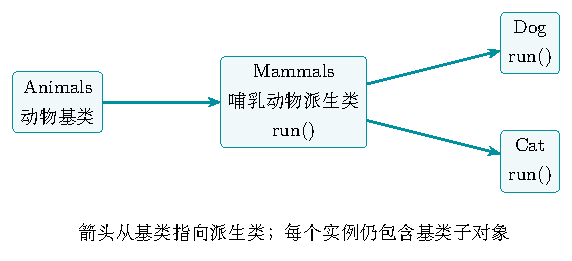
\includegraphics[width=0.7\textwidth]{inheritance_revised.pdf}
    \caption{类的继承} % 图片标题
    \label{fig:A111} % 图片标签，用于引用
\end{figure}

如图\ref{fig:A111}所示，派生类从基类中继承了数据成员和成员函数，并可以添加新的成员。
派生类可以重写基类中的成员虚函数，从而实现新的功能。
派生类可以重载基类中的运算符，从而实现新的运算。

下面按 public 继承、普通成员访问来比较（友元按授权另行处理）。protected 的派生类访问还受对象类型等规则约束，不能理解成对任意基类对象都随意访问。
这张表和"类的基本概念"中的是同一张，这里从继承的视角再看一次——重点关注"派生类"这一行：

\begin{center}
    \begin{tabular}{cccc}
        \toprule[1.5pt]
        访问位置 & public 成员 & private 成员 & protected 成员 \\
        \midrule[1pt]
        同一个类 & yes & yes & yes \\
        派生类 & yes & no & yes \\
        类外部 & yes & no & no \\
        \bottomrule[1.5pt]
    \end{tabular}
\end{center}

继承可以用下面的写法实现：

\Needspace{9\baselineskip}
\begin{example}
抽象基类与两个派生类：
\lstinputlisting[language=C++,numbers=left,numberstyle={\color{gray}\tiny}]{examples/class-basics-demo/inheritance.cpp}


从本卷目录进入 \path{examples/class-basics-demo}，保存的源码就是 \texttt{inheritance.cpp}。
\begin{tbash}
g++ -std=c++17 -Wall -Wextra -pthread inheritance.cpp -o /tmp/cpp-demo
/tmp/cpp-demo
\end{tbash}
先看到基类、再看到派生类的构造提示；下一道练习会通过基类指针调用面积函数。
\end{example}

\begin{note}
继承方式有三种：\texttt{public}、\texttt{protected}、\texttt{private}（\texttt{class} 默认 private，\texttt{struct} 默认 public），
它决定了基类成员在派生类中的访问权限上限。工程中绝大多数情况都用 \texttt{public} 继承，
另外两种仅作了解。含纯虚函数的抽象类不能直接实例化，只能作为基类使用。

另外注意初始化列表的写法：\textbf{基类构造函数写在成员之前}，成员之间按\textbf{声明顺序}初始化，
与列表里的书写顺序无关。写错顺序编译器会发出 \texttt{-Wreorder} 警告，如果成员之间存在初始化依赖，还会得到未定义的值。
\end{note}

\begin{conclusion}
重载（overload）与重写（override）仅一字之差，但完全是两回事：

\begin{itemize}
\item 重载 overload：同一作用域内的同名函数，参数列表不同，编译期由编译器选择版本，与继承无关；
\item 重写 override：派生类重新实现基类的 \texttt{virtual} 函数，函数签名必须相同，通过基类指针或引用调用时，根据对象实际类型决定调用哪个版本（多态），建议显式标注 \texttt{override} 让编译器帮忙检查；
\item 纯虚函数 \texttt{= 0}：基类只给接口不给实现，仍有纯虚函数没有最终实现的类是抽象类，不能实例化。纯虚函数也能在类外提供定义，这里先只把它作为接口使用。
\end{itemize}
\end{conclusion}

\begin{exercise}\label{ex:v1-cpp-inheritance}

在上例基础上，于 \texttt{main} 中创建 \texttt{Shape*} 数组分别指向 \texttt{Circle} 和 \texttt{Rectangle} 对象，
循环调用 \texttt{calArea()}，观察多态的调用结果。
\end{exercise}

 \subsubsection{模板}
在开发过程中，我们可能会遇到这样的场景：我们有一个函数或者类，但是它只适用于特定的数据类型，
比如\texttt{int}或者\texttt{double}。为了让这两种类型都可以调用函数，
就得把代码复制一遍，但这样做就造成了代码冗余，不利于维护。这时候就需要用到模板（\texttt{template}）。

模板是C++中一个重要的特性，它允许我们定义一个类或函数，使其可以接受不同的数据类型或者不同的参数。
模板的定义和使用都比较复杂，这里只介绍最基本的用法。
\textbf{函数模板}用 \texttt{template} 加尖括号声明一个类型参数（习惯命名为 \texttt{T}），之后 \texttt{T} 就可以像普通类型一样使用。语法如下：
\begin{tcode}
template<class T>
T function(T a){
    return a;
}
\end{tcode}

这里的\texttt{class T}表示一种数据类型，可以是任意类型。
在函数的定义中，\texttt{T}可以作为函数的参数，也可以作为函数的局部变量。在使用函数模板时，需要首先进行函数的实例化。

\Needspace{9\baselineskip}
\begin{example}
函数模板的实例化与调用：
\lstinputlisting[language=C++,numbers=left,numberstyle={\color{gray}\tiny}]{examples/class-basics-demo/function-template.cpp}


从本卷目录进入 \path{examples/class-basics-demo}，保存的源码就是 \texttt{function-template.cpp}。
\begin{tbash}
g++ -std=c++17 -Wall -Wextra -pthread function-template.cpp -o /tmp/cpp-demo
/tmp/cpp-demo
\end{tbash}
这里输出 1 和 10。实例化把模板参数换成具体类型，调用才执行函数体。
\end{example}

模板的优点：
\begin{enumerate}
    \item 代码重用性高：可以定义一个通用的函数，然后根据需要实例化不同的类型，实现代码的重用。
    \item 类型安全：不符合类型要求的用法通常能在编译时发现，而不是等运行时猜数据是什么。
    \item 效率高：编译器可以针对具体类型优化；实际速度仍要看算法与使用方式。
\end{enumerate}

\textbf{类模板}：
类模板的语法和函数模板类似，只不过在类名而不是函数名前面加上关键字\texttt{template}。
在普通类中也可以添加成员函数模板，只需要在函数名前面加上关键字\texttt{template}即可。

\Needspace{9\baselineskip}
\begin{example}
类模板的基本写法：
\lstinputlisting[language=C++,numbers=left,numberstyle={\color{gray}\tiny}]{examples/class-basics-demo/class-template.cpp}


从本卷目录进入 \path{examples/class-basics-demo}，保存的源码就是 \texttt{class-template.cpp}。
\begin{tbash}
g++ -std=c++17 -Wall -Wextra -pthread class-template.cpp -o /tmp/cpp-demo
/tmp/cpp-demo
\end{tbash}
这里输出 1 2.5，同一个类模板按两个类型参数组成了这个对象。
\end{example}

模板参数除了类型，还可以是\textbf{编译期常量}（非类型模板参数），常用于指定数组长度这类编译期就要确定的值：

\Needspace{9\baselineskip}
\begin{example}
非类型模板参数：
\lstinputlisting[language=C++,numbers=left,numberstyle={\color{gray}\tiny}]{examples/class-basics-demo/constant-template.cpp}


从本卷目录进入 \path{examples/class-basics-demo}，保存的源码就是 \texttt{constant-template.cpp}。
\begin{tbash}
g++ -std=c++17 -Wall -Wextra -pthread constant-template.cpp -o /tmp/cpp-demo
/tmp/cpp-demo
\end{tbash}
这里输出 42，N 在编译时已经确定。
\end{example}

在\texttt{template}后面，可以定义多个类型参数，用逗号分隔。需要注意的是，类中的函数模板需要在头文件中实现，
这使编译器在需要实例化时看得到定义。也可以显式实例化后分离编译，但初学阶段先把定义放进头文件，省去链接时找不到实现的麻烦。
对于类模板也可以实现继承和多态，与普通类相同，这里不再展开，感兴趣的同学可以自行探索。

\textbf{模板的实例化}：
模板的实例化指的是将模板定义和具体的模板参数绑定在一起，生成一个具体的类或函数。
写 \texttt{A<int, double>} 时，编译器会根据尖括号里的参数生成对应的版本。模板参数可以填两类东西：

\begin{enumerate}
    \item 具体类型：如\texttt{int}、\texttt{double}等基本类型，\texttt{struct}、\texttt{class}、\texttt{union}等复合类型，以及指针和引用类型；
    \item 编译期可以确定的常量：字面常量、宏、\texttt{constexpr}，对应上面的非类型模板参数。
\end{enumerate}

平时我们写的 \texttt{function<int>(10)} 其实叫\textbf{隐式实例化}——用到时才生成；
也可以在代码里写 \texttt{template class A<int, double>;} 主动要求编译器立刻生成，这叫\textbf{显式实例化}，
常用于模板分离编译的场景，初学阶段了解即可。

除此之外，还有一种变参模板，它可以接受任意数量的类型参数，但是在实例化时，必须指定具体的类型。
这种情况比较复杂，这里不再展开。

\begin{note}
对变参模板感兴趣的同学可以自行探讨：

\url{https://blog.csdn.net/fl2011sx/article/details/128077440}
\end{note}

\begin{exercise}\label{ex:v1-cpp-template}

编写函数模板 \texttt{myMax}，返回两个同类型参数中较大的一个，分别用 \texttt{int}、\texttt{double} 测试，
并尝试用 \texttt{myMax(1, 2.5)} 调用，观察编译器的报错信息，思考为什么。再运行 class-template.cpp 与 constant-template.cpp，分别指出类型参数与非类型参数；不能把运行时读入的整数直接当成编译期 N。
\end{exercise}
